\section{Résultats}

Cette section reprend, dans un premier temps, les résultats des analyses faites sur les parties aériennes et racinaires des plantes des six variétés étudiées.
Ensuite sont présentés les modélisations de systèmes racinaires de sorgho réalisées par ArchiSimple sur base des paramètres estimés.
Tous les codes Rmd écrits en vue de l'obtention des graphes présentés sont accessible sur \href{https://github.com/ndegives/Memoire}{Github}.
De même que les rapports au format HTML liés à ces codes.

\subsection{Partie aérienne}

Les rendements en matière sèche des différentes variétés de sorgho considérées en 2020, 2021 et 2022 figure sur la figure \ref{fig:rendement}.
Un diagramme ombrothermique reprenant température et précipitation observés durant les trois durées de culture est disponible en annexe \ref{an:aerial}


\begin{figure}[ht]
\centering
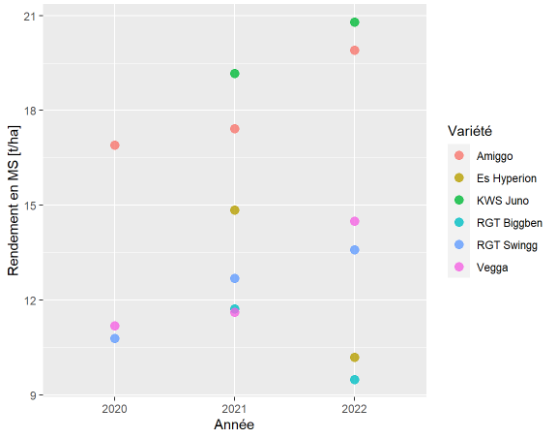
\includegraphics[width=0.6\textwidth]{Image/rendement.png}
\caption{Rendement des parties aériennes de plant de sorgho en fonction de l'année et de la variété}
\label{fig:rendement}
\end{figure}

Ce type de donnée peut être modélisé à l'aide du modèle à deux facteurs catégoriels et une réponse quantitative (ANOVA2) suivant :
\begin{equation}
    Y_{ijk} = \mu + \alpha_{i} + \beta_{j} + \gamma_{ij} + \epsilon_{ijk}
\end{equation}
avec :
\begin{itemize}
    \item $\mu$ : la moyenne générale
    \item $\alpha_i$ : effet de la variété i 
    \item $\beta_j$ : effet de l'année j
    \item $\gamma_{ij}$ : effet d'interaction entre variétés et année
    \item $\epsilon_{ijk}$ : la fluctuation aléatoire entre l'observation k et la moyenne du traitement. 
\end{itemize}

Malheureusement, n'ayant qu'une seule donnée par traitement, le cas d'un plan sans répétition se présente.
Afin de pouvoir tester les facteurs de variétés et d'années, il est nécessaire de supposer un effet d'interaction nul, or, il semble y en avoir un au vu de la figure \ref{fig:rendement}.
Le modèle serait dès lors largement faussé et ne sera donc pas développé.
On peut toutefois remarquer que les variétés Amiggo et Juno paraissent se démarquer des autres par des rendements relativement plus élevés que les autres.

\subsection{Caractérisation de l'architecture racinaire}

Cette section est dédiée au développement des estimations des cinq paramètres principaux précédemment décrits.
D'autres paramètres de ArchiSimple (EL, dSem, dAdv) sont également détaillés, car ceux-ci occupent une place centrale au vu du fonctionnement du modèle.
Les autres paramètres, provenant d'échantillons ou source comme décrit préalablement, ne seront pas différenciés entre variétés ni détaillés dans ce travail.
Ceux-ci sont, pour la plupart, calculés comme la moyenne observée sur tous les échantillons.
Seul CVDD est estimé comme la relation linéaire entre la valeur absolue des résidus du modèle DIDm et les valeurs estimées par celui-ci.
Les graphes et tableaux développant cette régression linéaire sont disponibles en annexe \ref{an:CVDD}.
Les paramètres n'ayant pas pu être estimés (représenté par le / dans le tableau \ref{tab:archisimple}) sont assignés à des valeurs arbitraires tout en restant cohérents avec l'ordre de grandeur du paramètre en question.

\subsubsection{Dmin : Le diamètre minimal}

La figure \ref{fig:boxplot Dmin} représente les distributions de la latérale la plus fine de chaque racine nodale en fonction de la variété.

\begin{figure}[ht]
\centering
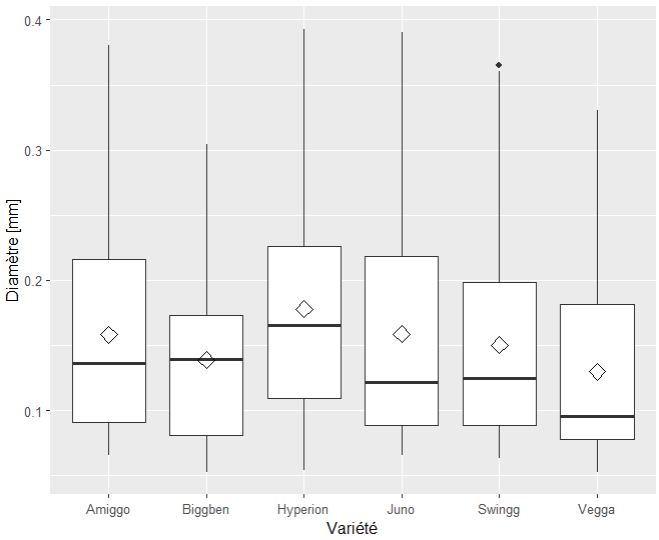
\includegraphics[width=0.5\textwidth]{Image/boxplot Dmin.png}
\caption{Box-plot de la latérale la plus fine pour chaque racine nodale en fonction de la variété}
\label{fig:boxplot Dmin}
\end{figure}

Les distributions semblent visuellement similaires.
Tant les valeurs moyennes et médianes que la largeur des boxplots sont semblables pour chaque variété.
Toutefois, les variétés Biggben, Hyperion et Vegga sont légèrement décalées par rapport aux trois autres.
Le résultat du test ANOVA est qu'au moins une variété a un Dmin significativement différent des autres.
Le tableau de ce test ainsi que la vérification des hypothèses sous-jacentes au modèle sont disponibles en annexe \ref{an:Dmin}.
Le modèle utilisé pour estimer et comparer ces distributions de Dmin est le modèle à un facteur catégoriel fixe suivant :
\begin{equation}
    Y_{ij} = \mu_{A}+\delta_{i}+\epsilon_{ij} \quad \text{avec :} \delta_{i}=\mu_{i}-\mu_{A} \, \text{et} \, \mu_{i} = \text{la moyenne de la variété i}
\end{equation}

Les résultats du modèle sont repris dans la table \ref{tab:summary Dmin} ci-dessous et montrent que seule la variété Vegga, pour laquelle le $\delta_{V}$ est significativement différent de 0 (p-valeur < $\alpha$ = 0.05), a un effet sur le Dmin.

\begin{table}[ht]
    \centering
    \caption{Summary du modèle pour estimer Dmin}
    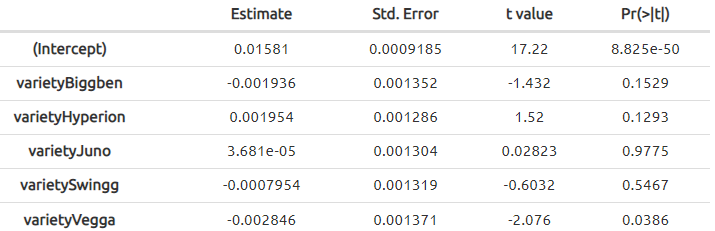
\includegraphics[width=0.75\textwidth]{Image/summary Dmin.png}
    \label{tab:summary Dmin}
\end{table}

La valeur de Dmin retenue pour l'estimation du paramètre Dmin est alors l'estimation du modèle pour la variété Vegga et la moyenne arithmétique des cinq autres variétés pour les autres, soit :

\begin{equation}
    D_{min} = 
    \begin{cases}
        \mu_{V} = \mu_{A}+\delta_{V} = 0.1297 [mm] & \text{pour la variété Vegga} \\
        \frac{\mu_{A}+\mu_{B}+\mu_{H}+\mu_{J}+\mu_{S}}{5}=0.1567 [mm] & \text{pour les autres variétés}
    \end{cases}
\end{equation}

\subsubsection{Dmax : le diamètre maximal}

Les distributions des diamètres de racines nodales en fonction de la variété sont présentées dans la figure \ref{fig:boxplot Dmax}.

\begin{figure}[ht]
\centering
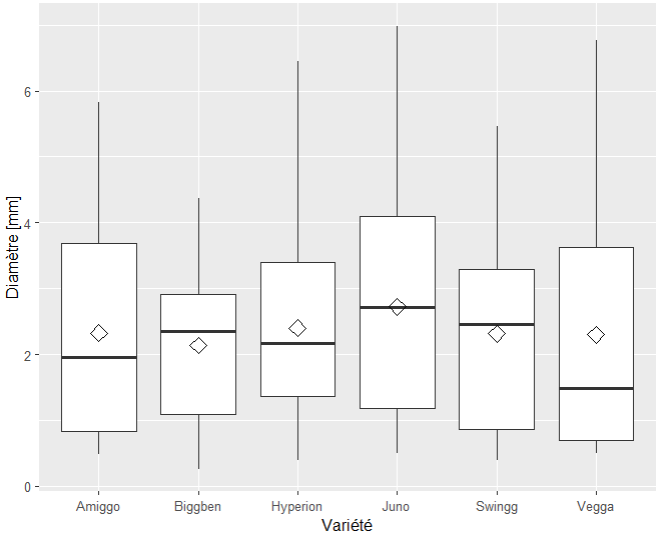
\includegraphics[width=0.5\textwidth]{Image/boxplot Dmax.png}
\caption{Box-plot des diamètres de racines nodales en fonction de la variété}
\label{fig:boxplot Dmax}
\end{figure}
\newpage

Similairement à ce qui a été observé pour Dmin, la distribution des diamètres des racines nodales est fortement similaire pour les six variétés.
Cet aperçu visuel est dans ce cas-ci confirmé par le test ANOVA (table \ref{tab:anova Dmax}) qui confirme l'égalité des distributions de diamètre de racines nodales des différentes variétés (p-valeur > $\alpha$ = 0.05).

\begin{table}[!ht]
    \centering
    \caption{Anova du modèle pour estimer Dmax}
    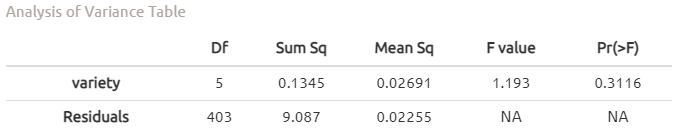
\includegraphics[width=0.75\textwidth]{Image/anova Dmax.png}
    \label{tab:anova Dmax}
\end{table}

L'estimation du paramètre Dmax sera dès lors la même pour les six variétés.
Celui-ci sera alors égal au diamètre maximum observé au sein de tous les échantillons, soit : $D_{max} = 6.984537$ mm.
Le modèle (non signifiatif dans ce cas) est développé en annexe \ref{an:Dmax} ainsi que les tests sur les hypothèses du modèle.

\subsubsection{Drange : la gamme de diamètres}

Les boxplots de Drange pour les six variétés sont présentés figure \ref{fig:boxplot Drange} ci-dessous.
On retrouve, à nouveau, beaucoup de similitudes entre les variétés et le test de variance du modèle (table \ref{tab:anova Drange}) ne laisse pas croire à une différence significative entre les variétés.
Les hypothèses relatives à l'utilisation du modèle sont présentées en annexe \ref{an:Drange}.

\begin{figure}[ht]
\centering
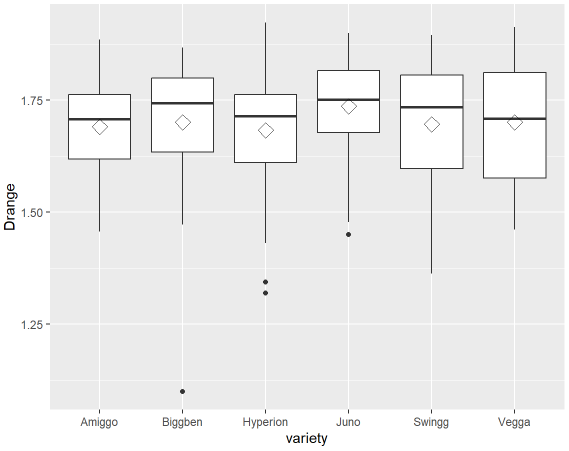
\includegraphics[width=0.5\textwidth]{Image/boxplot Drange.png}
\caption{Box-plot de Drange en fonction de la variété}
\label{fig:boxplot Drange}
\end{figure}

\begin{table}[ht]
    \centering
    \caption{ANOVA du modèle pour estimer Drange}
    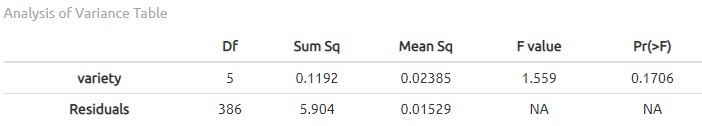
\includegraphics[width=0.75\textwidth]{Image/anova Drange.png}
    \label{tab:anova Drange}
\end{table}

Le résultat du calcul réalisé pour Drange ($2*(D_{max}-D_{min})/(D_{max}+D_{min})$) correspond au coefficient de variation des diamètres.
Ce coefficient permet principalement de comparer la variation au sein de données de moyennes différentes.
Drange n'est pas un paramètre requis en input de ArchiSimple.
L'estimation de celui-ci offre toutefois une vision globale des diamètres des différents systèmes racinaires qui, dans ce cas, seront donc considérés identiques avec un Drange de 1.7011.

\subsubsection{IBD : La distance entre latérales}

Les Boxplots des distances inter-primordium en fonction de la variété est présenté ci-dessous dans la figure \ref{fig:boxplot IBD}.

\begin{figure}[ht]
\centering
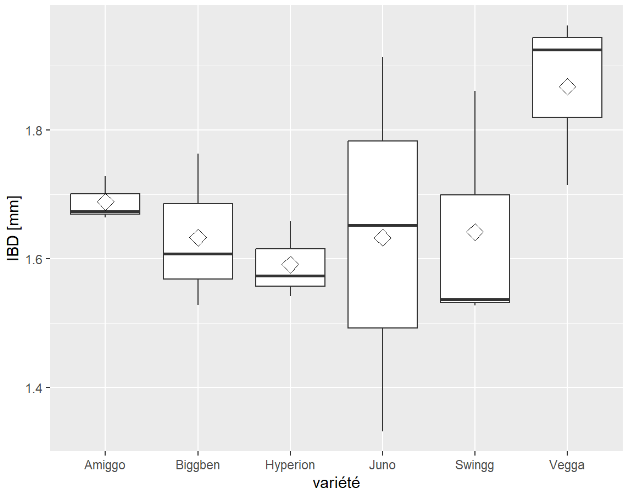
\includegraphics[width=0.5\textwidth]{Image/boxplot IBD.png}
\caption{Box-plot de IBD en fonction de la variété}
\label{fig:boxplot IBD}
\end{figure}

Les distributions, notamment celle pour la variété Vegga sont assez différentes dans ce cas.
Néanmoins, le test ANOVA (table \ref{tab:anova IBD}) n'indique pas de différence significative entre variétés.

\begin{table}[ht]
    \centering
    \caption{Anova du modèle pour estimer IBD}
    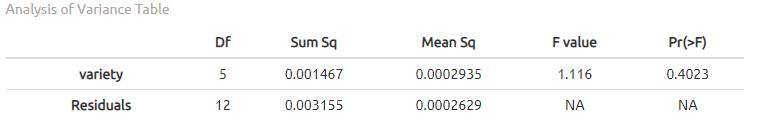
\includegraphics[width=1\textwidth]{Image/anova IBD.png}
    \label{tab:anova IBD}
\end{table}

La figure \ref{fig:inférence IBD} illustre les estimations faites par le modèle ANOVA sur le paramètre IBD.
Celles-ci sont relativement semblables pour toutes les variétés excepté Vegga qui, à nouveau, a une estimation plus élevée.
Des contrastes ont été réalisés afin d'avoir un test statistique plus spécifique à la variété Vegga.
Ces contrastes confirment une fois de plus que les estimations pour les différentes variétés ne peuvent pas être considérées comme étant différentes pour un niveau de confiance de $\alpha = 0.05$.

\begin{figure}[ht]
\centering
\includegraphics[width=0.85\textwidth]{Image/inférence IBD.png}
\caption{Inférence et contrastes Vegga pour IBD}
\label{fig:inférence IBD}
\end{figure}

Dès lors qu'aucun test n'indique un rejet de l'hypothèse d'égalité des moyennes entre variétés, celles-ci auront la même estimation moyenne de distance entre latérales soit : $IBD=1.6761 mm$.

\subsubsection{DIDm : le ratio Dfillle/Dmère}

La figure \ref{fig:plot DIDm} met en relation les diamètres de racines latérales avec le diamètre de leur racine parente par variété ainsi que les régressions linéaires qui en découlent.
Les droites de régressions linéaires semblent à priori significativement différentes pour chaque variété indiquant un effet de la variété, du diamètre de la racine mère et de l'interaction entre les deux sur le diamètre des racines latérales.
La table ANOVA \ref{tab:anova DIDm} confirme que ces effets sont significatifs.
\newpage

\begin{figure}[ht]
\centering
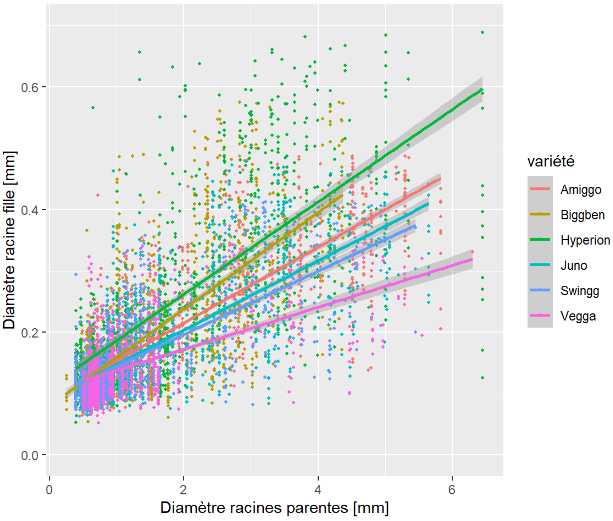
\includegraphics[width=0.6\textwidth]{Image/plot DIDm.png}
\caption{Plot du diamètre des racines fille par rapport à leur racine mère en fonction de la variétés }
\label{fig:plot DIDm}
\end{figure}

\begin{table}[ht]
    \centering
    \caption{Anova du modèle pour estimer DIDm}
    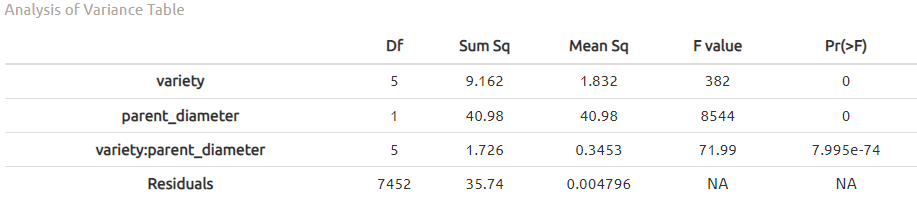
\includegraphics[width=1\textwidth]{Image/anova DIDm.png}
    \label{tab:anova DIDm}
\end{table}

Le modèle linéaire générale utilisé est le suivant : 
\begin{equation}
Y_{ij}=\beta_{0}+\beta_{1}*X_{ij}+\alpha_{i}+\gamma_{i}*X_{ij}+\epsilon_{ij}
\end{equation}
Avec : 
\begin{itemize}
    \item $\beta_{0}$ = l'intercepte de la régression linéaire de Amiggo.
    \item $\beta_{1}$ : effet du diamètre mère sur le diamètre fille pour Amiggo.
    \item $\alpha_{i}$ : effet de la variété sur l'intercepte par rapport à Amiggo.
    \item $\gamma_{i}$ : effet d'interaction diamètre mère et variétés.
    \item $\epsilon_{ij}$ : les résidus du modèle.
\end{itemize}

Les estimations des paramètres du modèle sont présentés dans la table \ref{tab:summary DIDm}.
\newpage

\begin{table}[ht]
    \centering
    \caption{Summary du modèle pour estimer DIDm}
    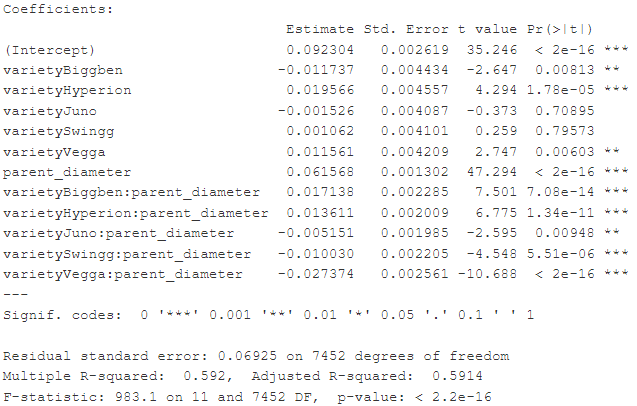
\includegraphics[width=0.68\textwidth]{Image/summary DIDm.png}
    \label{tab:summary DIDm}
\end{table}

Tous les paramètres semblent induire une différence notable dans l'estimation, à l'exception des paramètres des variétés Juno et Swingg.
Cette similitude s'observe sur la figure \ref{fig:plot DIDm} ou les interceptes de ces deux variétés sont très proches.
La même conclusion peut être tirée de l'observation des contrastes en annexe \ref{an:DIDm}.
Les estimations de DIDm qui sera retenue pour le paramètre DIDm sera l'estimation du modèle pour les différentes variétés telles que repris dans la table \ref{tab:emmeans DIDm}

\begin{table}[ht]
    \centering
    \caption{Estimations de DIDm}
    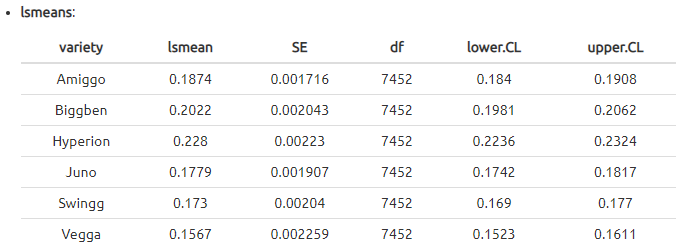
\includegraphics[width=0.6\textwidth]{Image/lsmeans DIDm.png}
    \label{tab:emmeans DIDm}
\end{table}

\subsubsection{EL : l'élongation en fonction du diamètre}

EL correspond à la pente de la relation observée entre le diamètre des racines primaires et leur croissance.
La figure \ref{fig:EL} ci-dessous illustre les données provenant des échantillons en rhizotron ainsi que la régression linéaire estimée par la fonction lm() en R.
\newpage

\begin{figure}[ht]
\centering
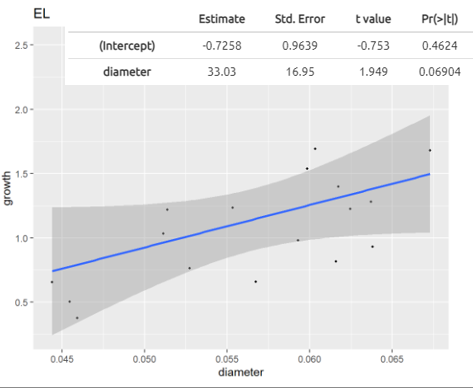
\includegraphics[width=0.55\textwidth]{Image/EL.png}
\caption{Plot et estimation de EL}
\label{fig:EL}
\end{figure}

L'estimation de EL utilisée dans le modèle pour les six variétés de sorgho correspond à la pente de la régression linéaire, soit $EL= 33.03$.
Le choix a été fait de ne pas imposer l'intercepte de cette courbe à passer par l'origine dès lors que le modèle se base sur un Dmin différent de 0 pour définir l'arrêt de la croissance d'une racine.
Par ailleur, cette relation peut également fournir une estimation de diamètre minimum au-delà duquel l'élongation racinaire est arrêtée (Dmin) en suivant le raisonnement suivant :
\begin{equation}
    \begin{cases}
        growth = -0.7258 + 33.03*diameter & \text{Équation de la droite} \\
        Dmin = \frac{0.7258}{33.03} = 0.02197 [cm] = 0.2197 [mm] & \text{Lorsque growth = 0}
    \end{cases}
\end{equation}

Cette estimation de Dmin est nettement supérieure à ce qui a été observé (0.2197 vs 0.1297 et 0.1567) et ne sera dès lors pas retenue pour l'estimation du paramètre Dmin.

\subsubsection{dSem et dAdv : les diamètres relatif de racines séminales et adventives}

Les diamètres relatifs des racines séminale et adventive, respectivement dSem et dAdv dans le modèle, sont mesurés sur base du diamètre maximal Dmax.
dSem est dès lors estimé par le ratio entre la moyenne des diamètres de racines primaires observées et Dmax soit $dSem=\frac{0.5648[mm]}{6.9845[mm]} = 0.08087$
L'estimation de dAdv est quant à elle faite sur base du ratio entre Dmax et la moyenne des diamètres de racines adventive observée, soit $dAdv = \frac{2.3795[mm]}{6.9845[mm]} = 0.3407$
Les deux paramètres sont supposés égaux pour toutes les variétés dès lors qu'il a été observé que les distributions des diamètres de racines primaires et nodales ne pouvaient pas être considérées comme significativement différentes auparavant.

\subsubsection{Tous les paramètres du modèle}

La table \ref{tab:esti.archisimple} reprend les estimations de tous les paramètres d'input du modèle.

\begin{table}[ht]
    \centering
    \caption{Estimation des paramètres de ArchiSimple}
    \includegraphics[width=0.75\textwidth]{Image/paramètre archisimple.png}
    \label{tab:esti.archisimple}
\end{table}

\subsection{Simulation d'architecture de système racinaire}
La durée de simulation a été fixée jusqu'à la fin de la phase végétative, soit environ 40 jours.
\cite{pellerinand_evaluation_1994} observaient que l'extension du système racinaire atteint un maximum quelques jours après la fin de la phase végétative chez le maïs.
Les systèmes racinaires générés par ArchiSimple sont présentés dans la figure \ref{fig:roots} ci-dessous.
\newpage

\begin{figure}[ht]
\centering
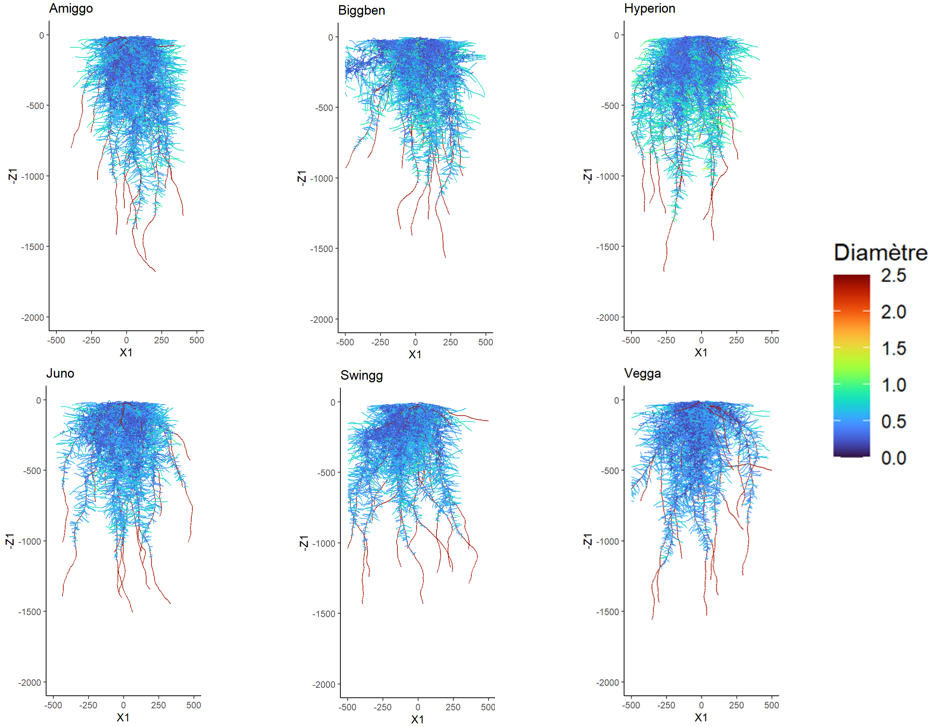
\includegraphics[width=1\textwidth]{Image/roots.png}
\caption{Résultats des modélisations des six variétés}
\label{fig:roots}
\end{figure}

On observe, comme décrit dans la littérature, un système racinaire construit avec des racines adventives de grands diamètres.
Celle-ci s'enfonce profondément dans le sol et donne lieu à des racines latérales qui permettent une meilleure exploration du sol.
Afin de voir comment se construisent ces systèmes racinaires, la figure \ref{fig:roots_day} affiche l'évolution du système racinaire depuis le 10ème jour jusqu'au 40ème par pas de temps de cinq jours pour la variété Amiggo.
\newpage

\begin{figure}[ht]
\centering
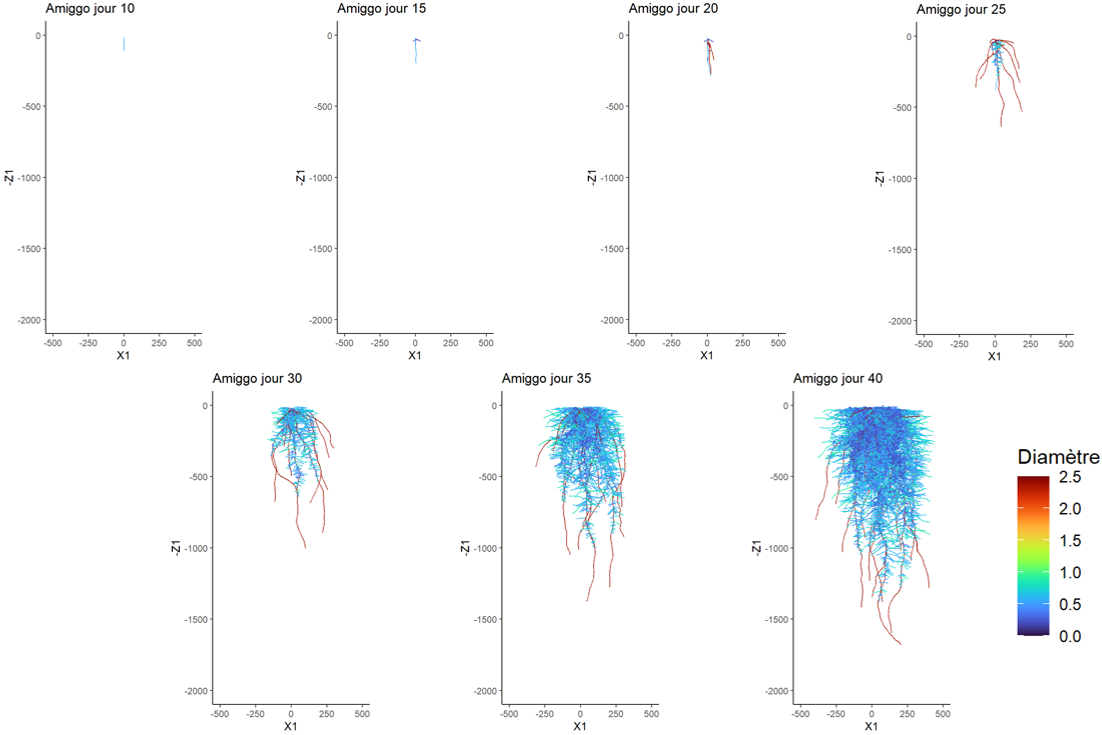
\includegraphics[width=1\textwidth]{Image/root_day.png}
\caption{Évolution de la modélisation tous les cinq jours pour Amiggo}
\label{fig:roots_day}
\end{figure}

Le sorgho ne développe, dans un premier temps, que sa racine primaire.
Au 15ème jour, la racine primaire s'est allongée et on observe un développement de quelques racines latérales sur la racine primaire.
Dès le vingtième jour, les racines nodales commencent à apparaître dans la modélisation.
Au jour 25, la racine primaire est plus ramifiée et certaines racines nodales sont plus longues que la racine primaire.
Après une trentaine de jours, on ne discerne plus la racine primaire, les racines nodales sont encore plus longues et possèdent des ramifications.
Finalement, jusqu'au jour 40, les racines nodales grandissent encore et se ramifient de plus en plus.
Ce développement correspond bien globalement à ce qui pourrait être observé sur un vrai système racinaire de sorgho.
